\section{Versuchsaufbau}
\label{sec:aufbau}

	\begin{wrapfigure}{r}{7cm}
		\centering
		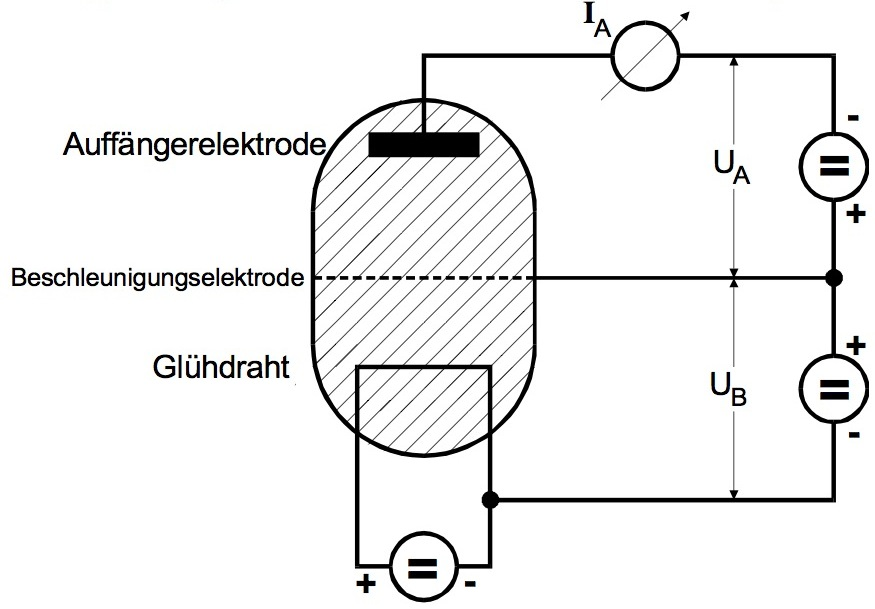
\includegraphics[width = 7cm]{img/aufbau.jpeg}
		\caption{Versuchsaufbau \cite{anleitung}. \label{fig:aufbau}}
	\end{wrapfigure}
	Der Franck-Hertz-Versuch ist in Abbildung \ref{fig:aufbau} schematisch Dargestellt.
	In einem evakuierten Gef"a"s verdampft ein Tropfen Quecksilber, sodass sich Quecksilberatome homogen in diesem verteilen.
	Der Druck des Quecksilberdampfes kann durch die Temperatur $T$ gesteuert werden.

	Im unteren Teil des Gef"a"ses befindet sich eine Gl"uhkathode aus Wolfram, die durch Gleichstrom erhitzt wird.
	Es treten auf Grund des gl"uhelektrischen Effektes Elektronen aus dem Material aus und bilden eine Elektronenwolke um den Wolframdraht.

	Zwischen Gl"uhkathode und einem, in der Mitte des Gef"a"ses befestigtem Drahtgitter, wird eine Spannung $U_\mathrm{B}$ angelegt, sodass die Elektronen in Richtung des Drahtgitters beschleunigt werden.

	Hinter dem Drahtgitter, im oberen Teil des Gef"a"ses befindet sich eine weitere Elektrode, die zum Drahtgitter ein negatives Potential $U_\mathrm{A}$ besitzt.
	Elektronen, die das Drahtgitter passieren und gen"ugend Energie besitzten, k"onnen das Potential $U_\mathrm{A}$ "uberwinden und als Auffangstrom $I_\mathrm{A}$ in der Elektrode gemessen werden.
	Langsame Elektronen werden dagegen zur"uck zum Drahtgitter gelenkt und von diesem absorbiert. 
	\\*

	\begin{wrapfigure}{r}{7cm}
		\centering
		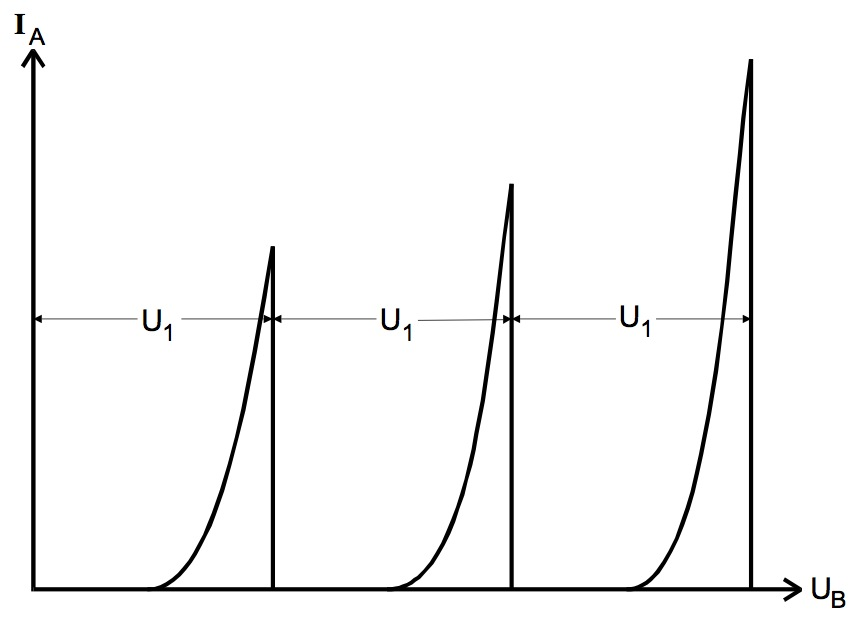
\includegraphics[width = 7cm]{img/strom-spannung.jpeg}
		\caption{Idealisiertes Strom-Spannungs-Diagramm \cite{anleitung}. \label{fig:strom-spannung}}
	\end{wrapfigure}

	Durch Erh"ohung der Beschleunigungsspannung $U_\mathrm{B}$ kann die kinetische Energie der Elektronen stetig erh"oht werden. Mit der Elektronenladung $e$ gilt
	\begin{equation}
		E_\mathrm{kin} = e \cdot U_\mathrm{B} \,.
	\end{equation}

	Bei konstanter Auff"angerspannung $U_\mathrm{A}$ erreichen dann mit steigender Spannung $U_\mathrm{B}$ immer mehr Elektronen die Auff"angerelektrode und der Strom $I_\mathrm{A}$ w"achst.

	Auf dem Weg durch das Gef"a"s sto"sen die Elektronen mit den Quecksilberatomen zusammen.
	Wenn sie nun gen"ugend kinetische Energie $E_\mathrm{kin} = \Delta E$ besitzen, sodass sie die Quecksilberatome anregen k"onnen, treten unelastische St"o"se auf.
	Die gesamte Energie der Elektronen geht dann in die Quecksilberatome "uber und der Strom $I_\mathrm{A}$ f"allt auf 0.
	Die kinetische Energie der Elektronen stimmt dann mit der Energiedifferenz $\Delta E$ zwischen Grundzustand und erstem angeregten Zustand des Quecksilberatoms "uberein.

	Durch weitere Erh"ohung der Beschleunigungsspannung $U_\mathrm{B}$ wiederholt sich dieser Prozess, sodass ein Strom-Spannungs-Diagramm, wie in Abbildung \ref{fig:strom-spannung} dargestellt, entsteht.
	Durch Messung des Abstandes $U_1$ zwischen zwei Strommaxima l"asst sich somit die Energiedifferenz $\Delta E$ bestimmen und es gilt

	\begin{equation}
		\Delta E = e \cdot U_1 \,.
	\end{equation}

	\subsection{Systematische Abweichungen}
	\label{subsec:abweichungen}
		Auf Grund verschiedener Effekte, die im Folgenden aufgef"uhrt sind, weicht die tats"achlich messbare Kurve von der idealisierten Kurve in Abbildung \ref{fig:strom-spannung} ab.

		\begin{itemize}
			\item Die Strom-Spannungs-Kuver ist um einen Wert $K$ verschoben.
			Dieser Wert $K$ bezeichnet das Kontaktpotential, welches auf Grund der verschiedenen Austrittsarbeiten des Kathoden- und des Gitterdrahtmaterials auftritt und durch das Fermi-Niveau $\Phi$ der Materialien bestimmt ist:

			\begin{equation*}
				K = \frac{1}{e} (\Phi_\mathrm{B} - \Phi_\mathrm{A})
			\end{equation*}

			\item Die Kurve erscheint abgeflacht und verbreitert, weil die Elektronen nicht mit konstanter Geschwindigkeit aus dem Gl"uhdraht austreten.
			Die Elektronen besitzen stattdessen ein Energiespektrum, welches als Fermi-Dirac-Verteilung bezeichnet wird.
			Dadurch f"allt der Auffangstrom $I_\mathrm{A}$ nach einem Maximum nicht mehr unstetig auf den Wert 0 ab, sondern n"ahert sich stetig einem Minumum, das nicht 0 ist.

			\item Die Wahrscheinlichkeit, dass die Elektronen mit Quecksilberatomen kollidieren h"angt stark vom Dampfdruck $p$ des Quecksilbergases ab.
			Dieser legt die freie Wegl"ange $\overline{w}$ fest, die ein Elektron durchschnittlich zur"ucklegen muss, um mit einem Quecksilberatom zu kollidieren.

			Falls die Wegl"ange $\overline{w}$ gr"o"ser als die Dimension $a$ der Versuchsapparatur ist, treten kaum Kollisionen auf und eine Messung ist schwierig.
			Wenn die Wegl"ange $\overline{w}$ viel kleiner ist als $a$, treten zwischen den unelastischen St"o"sen viele elastische St"o"se auf, die mit starken Richtungs"anderungen verbunden sind.
			Dadurch verringert sich die Anzahl der Elektronen, die die Auffangelektrode erreichen und das Ergebnis wird verf"alscht.
		\end{itemize}

	\clearpage

\section{Durchf"uhrung}
\label{sec:durchfuehrung}
	\begin{figure}[h]
		\centering
		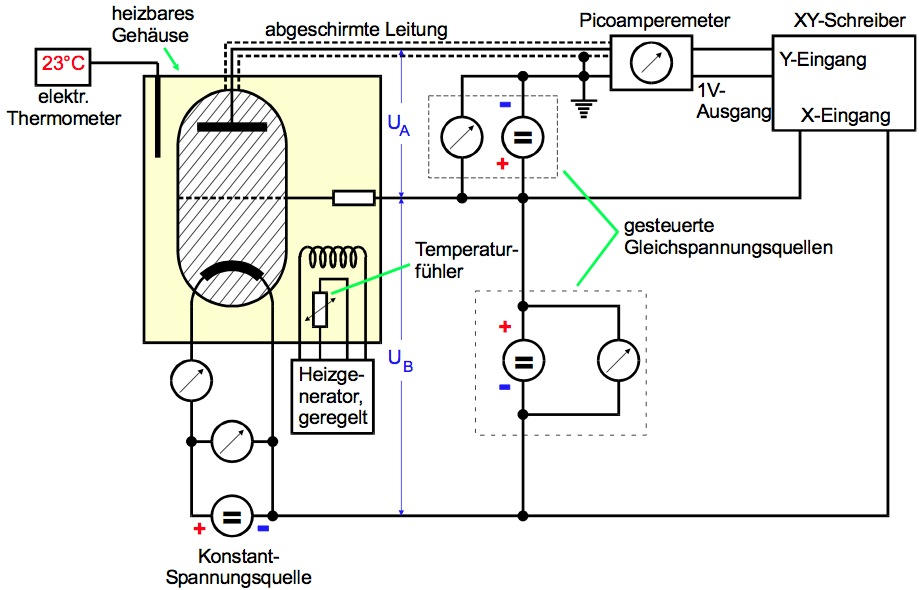
\includegraphics[width = 12cm]{img/aufbau-exakt.jpeg}
		\caption{Aufbau der hier verwendeten Apparatur \cite{anleitung}. \label{fig:aufbau-exakt}}
	\end{figure}

	Die hier verwendeta Apparatur ist in Abbildung \ref{fig:aufbau-exakt} dargestellt.
	Das gesamte, mit Quecksilberdampf bef"ullte Gef"a"s befindet sich in einem Blechgeh"ause, welches durch einen elektronischen Temperaturreglers erhitzt werden kann.
	Die Temperatur $T$ wird mit einem elektronischen Thermometer gemessen.
	Die Brems- und Beschleunigungsspannungen $U_\mathrm{A}$ und $U_\mathrm{B}$ k"onnen kontinuierlich von 0 auf $U_\mathrm{A} = \SI{11}{\volt}$ bzw. $U_\mathrm{B} = \SI{60}{\volt}$ geregelt werden.
	Dabei kann die Zeit $t$, in der geregelt wird zwischen $t = \SI{30}{\second}$ und $t = \SI{5}{\minute}$ variiert werden.

	